
\section{Illustrative examples}

\textit{Provide at least one illustrative example to demonstrate the major
functions of your software/code.}

\textit{\textbf{Optional}: you may include one explanatory  video or screencast that will appear next to your article, in the right hand side panel. Please upload any video as a single supplementary file with your article. Only one MP4 formatted, with 150MB maximum size, video is possible per article. Recommended video dimensions are 640 x 480 at a maximum of 30 frames / second. Prior to submission please test and validate your .mp4 file at  \url{http://elsevier-apps.sciverse.com/GadgetVideoPodcastPlayerWeb/verification} . This tool will display your video exactly in the same way as it will appear on ScienceDirect. }

\begin{table}[!h]
\begin{tabular}{|r|r|r|r|r|}
  \hline
  \textbf{Nr.}&  \textbf{Path no 1}&  \textbf{Path no 2}&  \textbf{Path no 3}&  \textbf{Path no 4}\\
  \hline
  1& -0.518& -0.550& 0.567& 0.501\\
  \hline
  2& -0.228& -0.259& -0.377& 0.864\\
  \hline
  3& 0.454& 0.420& -0.069& -0.805\\
  \hline
  4& 0.103& -0.434& 0.373& -0.043\\
  \hline
  5& -0.445& -0.160& 0.434& 0.171\\
  \hline
  6& -0.105& -0.226& 0.239& 0.093\\
  \hline
  7& 0.136& -0.222& -0.102& 0.188\\
  \hline
  8& 0.446& -0.122& -0.009& -0.316\\
  \hline
  9& 0.367& 0.149& -0.377& -0.139\\
  \hline
  10& 0.083& -0.012& -0.035& -0.037\\
  \hline
  11& 0.184& -0.042& 0.102& -0.244\\
  \hline
  12& -0.381& 0.166& 0.365& -0.149\\
  \hline
  13& -0.318& 0.319& 0.165& -0.166\\
  \hline
\end{tabular}

\caption{Test}
\label{testTable}
\end{table}

\begin{figure}[!h]
\begin{tikzpicture}
\begin{axis}[
    title={Score dependence on iteration},
    xlabel={Iteration},
    ylabel={Score},
    legend pos=outer north east,
    ymajorgrids=true,
    grid style=dashed,
]

\addplot[
    color=blue,
    mark=square
    ]
    table[x=Nr.,y=Path1]
    {Fig/Score.dat};
\addplot[
    color=red,
    mark=square
    ]
    table[x=Nr.,y=Path2]
    {Fig/Score.dat};
\addplot[
    color=green,
    mark=square
    ]
    table[x=Nr.,y=Path3]
    {Fig/Score.dat};
\addplot[
    color=black,
    mark=square
    ]
    table[x=Nr.,y=Path4]
    {Fig/Score.dat};

    \legend{Path 1, Path 2, Path 3, Path 4}


\end{axis}
\end{tikzpicture}

\caption{Test}
\label{testFig}
\end{figure}

Odnośnik do rysunku~\ref{testPng}.

\begin{figure}[!h]
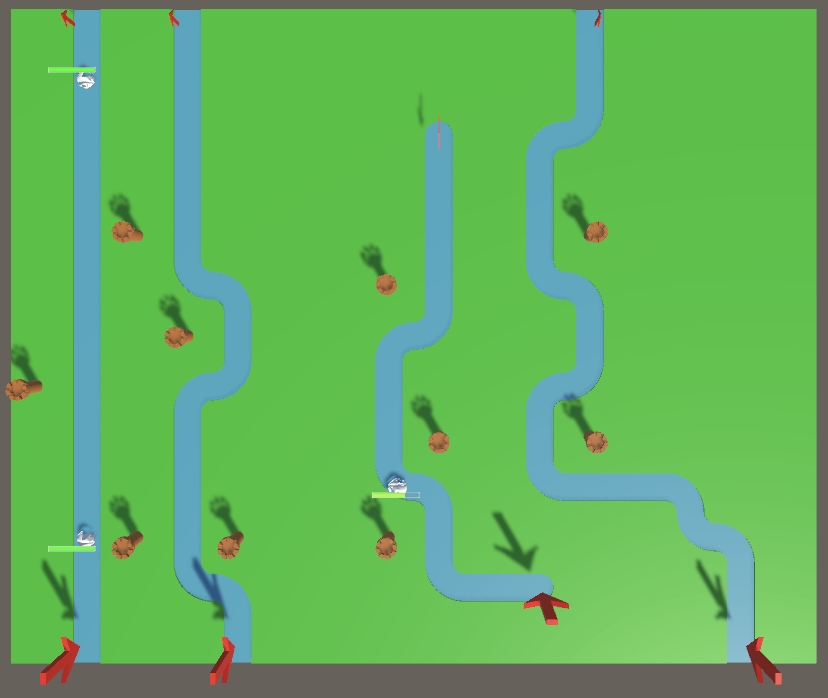
\includegraphics[width=6cm]{test.png}
\caption{Dołączanie rysunków png}
\label{testPng}
\end{figure}

\begin{figure}[!h]
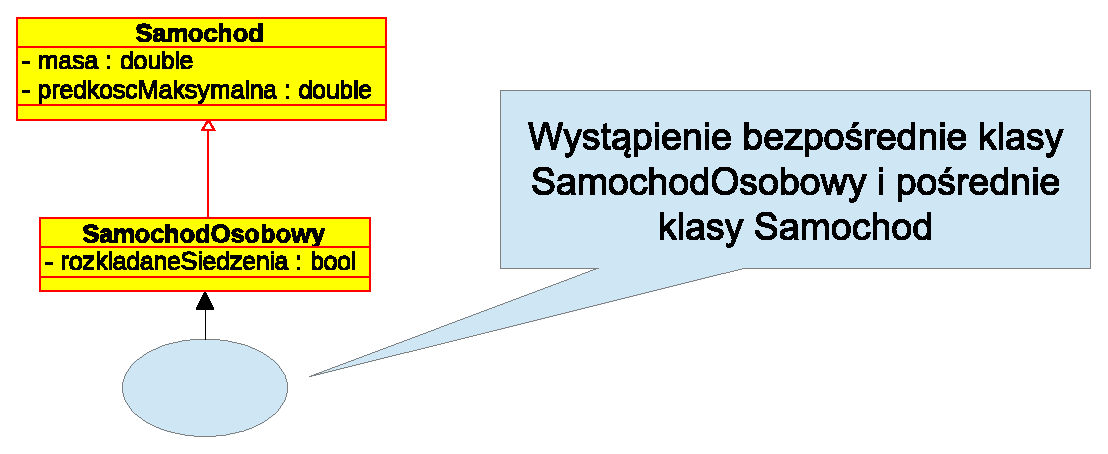
\includegraphics[width=9cm]{test.eps}
\caption{Dołączanie rysunków eps, przy eksporcie trzeba dać 'Zaznaczenie'}
\label{testEPS}
\end{figure}

Cytowanie literatury~\cite{council_of_the_eu_annex_2022}. Cytowanie wielu pozycji~\cite{polish_alternative_fuels_association_polish_nodate,buchanan_objectivity_1998}. Aby bibliografia się zaktualizowała należy skompilować latex-a (xelatex-a lub co tam aktualnie używasz), potem skompilować bibtex-a, a potem jeszcze dwa razy latex-a.

